\documentclass[12pt,a4paper]{article}
\usepackage[utf8]{inputenc}
\usepackage[spanish,es-tabla]{babel}
\usepackage{geometry}
\usepackage{graphicx}
\usepackage{multirow}
\usepackage{tabularx}
\usepackage{mathptmx}
\usepackage{fancyhdr}
\usepackage{array}
\usepackage[table]{xcolor}
\usepackage{titlesec}
\usepackage{setspace}
\usepackage{microtype}
\usepackage{lastpage}
\usepackage{booktabs}
\usepackage{enumitem}
\usepackage{amsmath}
\usepackage{amsfonts}
\usepackage{amssymb}

\graphicspath{{images/}{../images/}{./}}

\geometry{
    top=4.7cm,
    bottom=2.5cm,
    left=2.5cm,
    right=2.5cm,
    headheight=3.9cm,
    headsep=0.4cm
}

\setstretch{1.15}
\setlength{\parindent}{0pt}
\setlength{\parskip}{0.45em}
\setlength{\tabcolsep}{4pt}

\titleformat{\section}
  {\normalfont\fontsize{12}{14.5}\bfseries}{\thesection.}{0.6em}{\uppercase}
\titlespacing*{\section}
  {0pt}{1.8ex plus 0.4ex minus 0.2ex}{0.6ex plus 0.2ex}

\titleformat{\subsection}
  {\normalfont\fontsize{11.5}{13.5}\bfseries}{\thesubsection.}{0.5em}{}
\titlespacing*{\subsection}
  {0pt}{1.4ex plus 0.3ex minus 0.1ex}{0.4ex plus 0.1ex}

\titleformat{\subsubsection}
  {\normalfont\fontsize{10.5}{12.5}\bfseries\itshape}{\thesubsubsection.}{0.4em}{}
\titlespacing*{\subsubsection}
  {0pt}{1.1ex plus 0.2ex minus 0.1ex}{0.3ex plus 0.1ex}

\newcolumntype{Y}{>{\centering\arraybackslash}X}
\newcolumntype{L}{>{\raggedright\arraybackslash}X}
\newcolumntype{C}{>{\centering\arraybackslash}X}

\definecolor{headerblue}{RGB}{26, 54, 93}
\definecolor{darkblue}{RGB}{43, 108, 176}
\definecolor{lightgraybg}{RGB}{248, 248, 248}
\definecolor{tableheader}{RGB}{232, 238, 246}

\newcommand{\docCodigo}{TI-SIGE-ENT-F4-002}
\newcommand{\docVersion}{1.0}
\newcommand{\docProceso}{CONTROL DE CALIDAD / SEGURIDAD E INTEGRACIÓN}
\newcommand{\docElaboracion}{13/10/2026}
\newcommand{\docRevision}{13/10/2026}
\newcommand{\docTitulo}{PRUEBAS DE INTEGRACIÓN Y SEGURIDAD}
\newcommand{\docOrganizacion}{FACULTAD DE INGENIERÍA EN SISTEMAS, ELECTRÓNICA E INDUSTRIAL}
\newcommand{\docSubOrganizacion}{CARRERA DE INGENIERÍA DE SOFTWARE}

\newcommand{\encabezadofrecuente}{%
    \renewcommand{\arraystretch}{1.15}%
    \noindent\makebox[\textwidth][c]{%
    \begin{tabularx}{\textwidth}{|>{\centering\arraybackslash}m{2.8cm}|Y|>{\centering\arraybackslash}m{4.8cm}|}
        \hline
        \multirow{4}{2.8cm}{\centering\raisebox{-1.15cm}{
\includegraphics[width=2.5cm,height=2.0cm,keepaspectratio]{images/logo.png}}}
        & \textbf{\fontsize{9}{11}\selectfont \docOrganizacion} 
        & \textbf{\fontsize{8}{10}\selectfont CÓDIGO:} \fontsize{8}{10}\selectfont \docCodigo \\
        \cline{3-3}
        & \textbf{\fontsize{8.5}{10.5}\selectfont \docSubOrganizacion} 
        & \textbf{\fontsize{8}{10}\selectfont VERSIÓN:} \fontsize{8}{10}\selectfont \docVersion \\
        \cline{2-3}
        & \textbf{\fontsize{8}{10}\selectfont PROCESO:} \fontsize{8}{10}\selectfont \docProceso 
        & \textbf{\fontsize{8}{10}\selectfont ELABORACIÓN:} \fontsize{8}{10}\selectfont \docElaboracion \\
        \cline{2-3}
        & \textbf{\fontsize{8.5}{10.5}\selectfont \docTitulo} 
        & \textbf{\fontsize{8}{10}\selectfont ÚLTIMA REVISIÓN:} \fontsize{8}{10}\selectfont \docRevision \\
        \hline
    \end{tabularx}%
    }%
}

\pagestyle{fancy}
\fancyhf{}
\fancyhead[C]{\encabezadofrecuente}
\fancyfoot[C]{\fontsize{10}{12}\selectfont Página \thepage\ de \pageref{LastPage}}
\renewcommand{\headrulewidth}{0pt}

\begin{document}

\noindent{\fontsize{10.5}{12.5}\selectfont \textbf{Integrantes:} Heidi Villavicencio \quad$\vert$\quad Steeven Toala \quad$\vert$\quad Nixon Hurtado \quad$\vert$\quad Andrea Vásquez}

\vspace{0.25cm}

\section{Título}
\textbf{Denominación del Entregable:} Pruebas de Integración y Seguridad (Auditoría OWASP) -- Código EDT: 4.2

\section{Introducción}
El despliegue de una plataforma académica en un servidor público exige la validación rigurosa de las interfaces de comunicación entre componentes y la resistencia de las APIs frente a vectores de ataque conocidos. Iniciada el 13 de octubre de 2026, la actividad EDT 4.2 evalúa la integración de extremo a extremo entre los controladores Express v5, PostgreSQL 18 y MinIO S3, sometiendo simultáneamente la aplicación a una auditoría técnica de seguridad y pentesting orientada por el estándar internacional OWASP Top 10 API Security Risks.

\section{Objetivo}
\subsection{Objetivo General}
Ejecutar las pruebas de integración entre subsistemas y auditar la seguridad técnica del sistema SIGE bajo los lineamientos OWASP, certificando la protección de la información institucional.
\subsection{Objetivos Específicos}
\begin{itemize}[leftmargin=1.5em, itemsep=2pt]
    \item Validar la persistencia transaccional y rollback automático en flujos cruzados Express-PostgreSQL-MinIO.
    \item Evaluar los 10 riesgos de seguridad de APIs según OWASP Top 10.
    \item Verificar el endurecimiento (Hardening) de encabezados HTTP de seguridad (Helmet, HSTS, CSP, CORS).
    \item Realizar pruebas de simulación de escalación horizontal y vertical de privilegios RBAC.
\end{itemize}

\section{Alcance}
\subsection{Límites del Entregable (In-Scope)}
\begin{itemize}[leftmargin=1.5em, itemsep=2pt]
    \item Auditoría de endpoints de autenticación, persistencia y descarga de evidencias.
    \item Análisis estático de código (SAST) y pruebas dinámicas de penetración (DAST) en entorno local.
\end{itemize}
\subsection{Exclusiones (Out-of-Scope)}
\begin{itemize}[leftmargin=1.5em, itemsep=2pt]
    \item Ataques de denegación distribuida de servicio (DDoS) a nivel de infraestructura física de telecomunicaciones.
\end{itemize}

\section{Definiciones}
\begin{itemize}[leftmargin=1.5em, itemsep=2pt]
    \item \textbf{Pruebas de Integración:} Nivel del desarrollo de software donde los módulos individuales se combinan y se prueban como un grupo para validar sus interfaces.
    \item \textbf{OWASP (Open Web Application Security Project):} Comunidad global dedicada a mejorar la seguridad de las aplicaciones y software.
    \item \textbf{BOLA (Broken Object Level Authorization):} Vulnerabilidad donde un usuario puede manipular el identificador de un objeto para acceder a datos no autorizados.
    \item \textbf{HTTP Security Headers:} Encabezados HTTP (Content-Security-Policy, Strict-Transport-Security, X-Frame-Options) que mitigan ataques en el navegador.
\end{itemize}

\section{Responsabilidades}
\begin{itemize}[leftmargin=1.5em, itemsep=2pt]
    \item \textbf{Steeven Toala / Nixon Hurtado (Responsables EDT 4.2):} Ejecución de pruebas de integración, auditoría de seguridad y pentesting.
    \item \textbf{Andrea Vásquez (QA):} Verificación de respuestas seguras del cliente ante peticiones no autorizadas.
    \item \textbf{Ing. Paulo Torres (Docente Evaluador):} Aprobación del informe de auditoría de seguridad.
\end{itemize}

\section{Normativa Legal y Técnica}
\begin{itemize}[leftmargin=1.5em, itemsep=2pt]
    \item \textbf{OWASP API Security Top 10 (2023 Edition).}
    \item \textbf{ISO/IEC 27001:2022 (Control 8.28: Secure Coding).}
\end{itemize}

\section{Método, Políticas y Contenidos}
Se utilizó escaneo estático y pruebas dinámicas con Postman y OWASP ZAP. En la Figura \ref{fig:f4_02_sec} se presenta el esquema de integración y validaciones de seguridad evaluadas.

\begin{figure}[htbp]
    \centering
    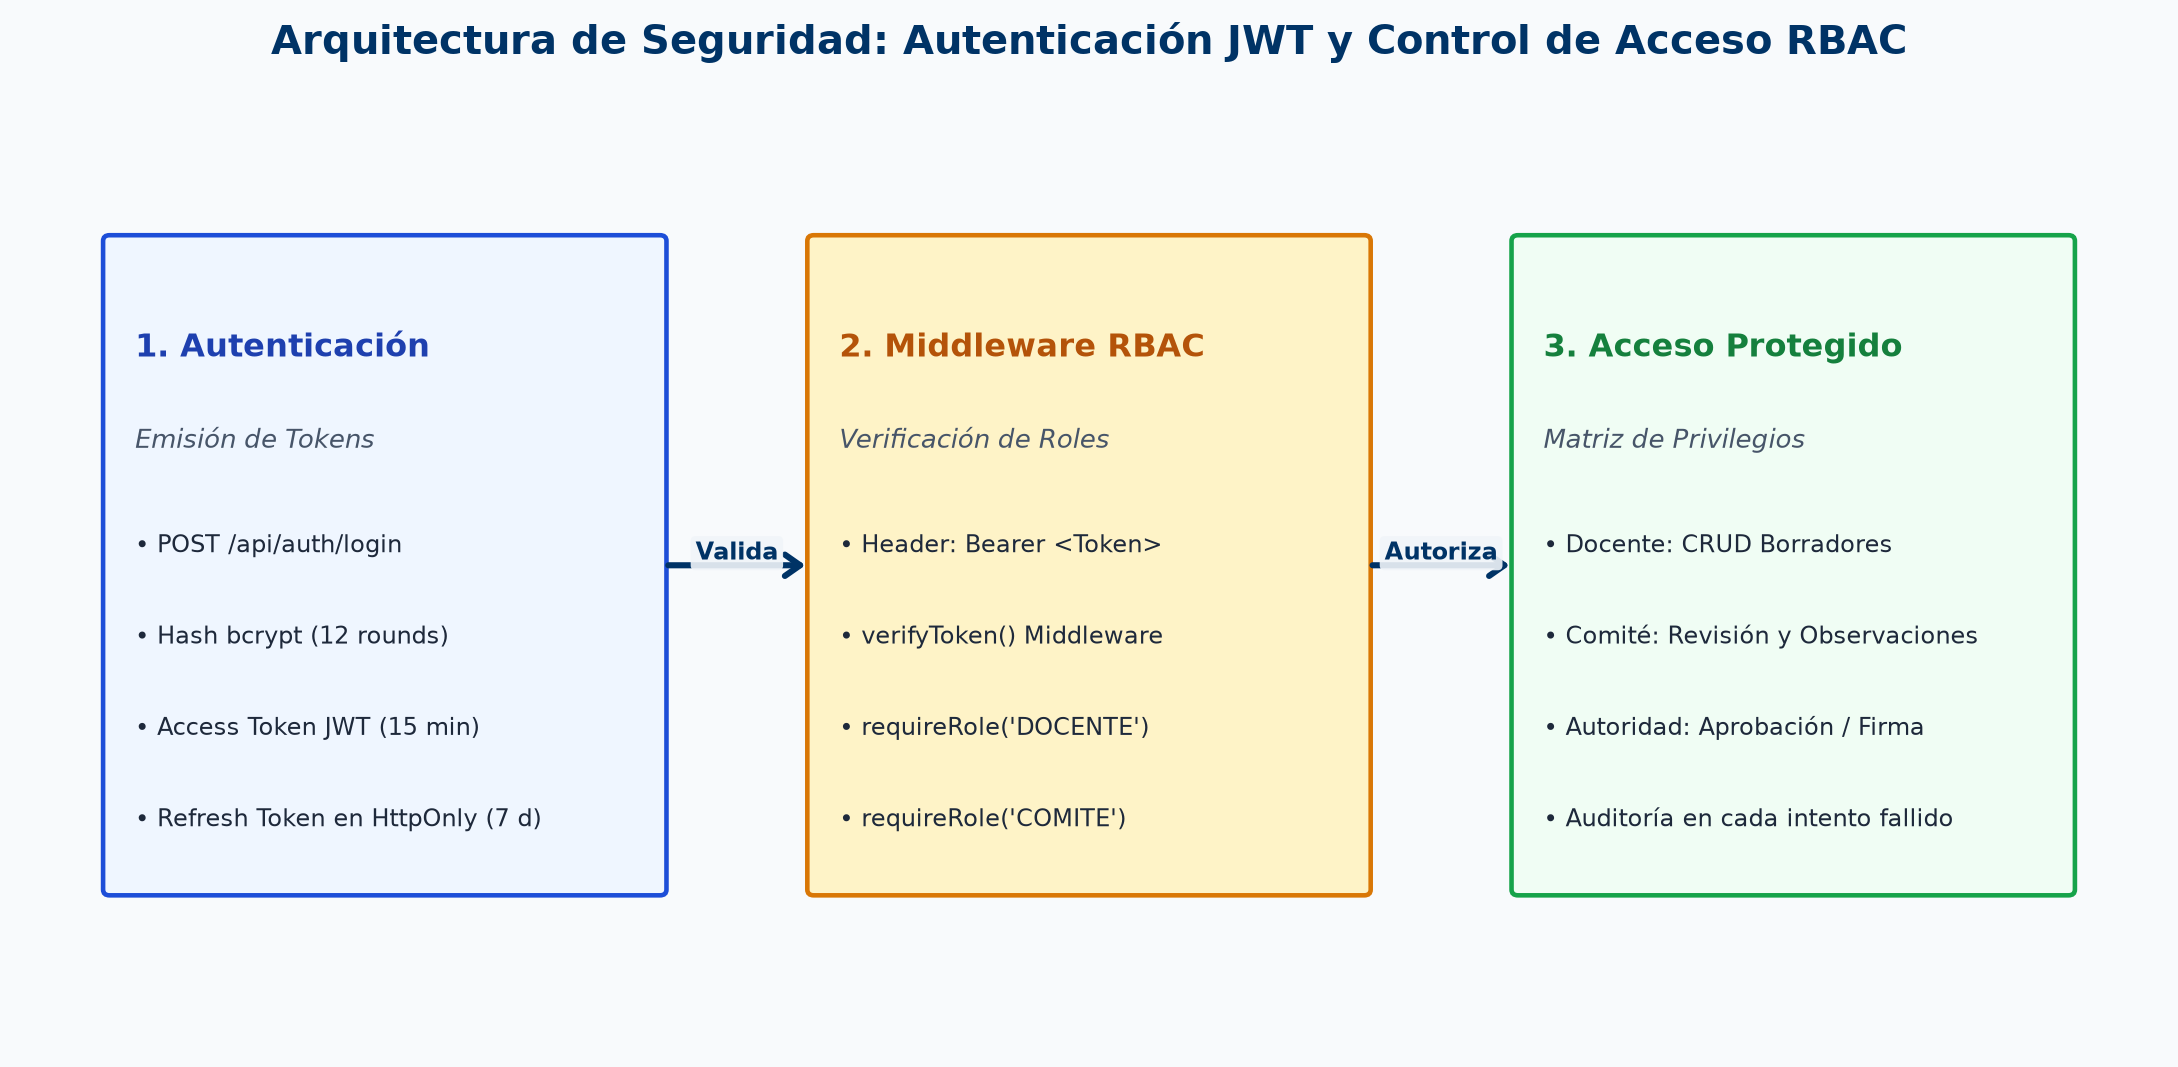
\includegraphics[width=0.88\textwidth,height=5.2cm,keepaspectratio]{images/f3_03_seguridad_jwt_rbac.png}
    \caption{Arquitectura de Pruebas de Integración y Mitigación de Vulnerabilidades OWASP.}
    \label{fig:f4_02_sec}
\end{figure}

\section{Descripción de actividades}
\subsection{Matriz de Auditoría OWASP API Security Top 10}
\begin{table}[htbp]
\centering
\small
\renewcommand{\arraystretch}{1.2}
\begin{tabularx}{\textwidth}{|c|>{\bfseries}m{3.2cm}|X|c|}
\hline
\rowcolor{tableheader}
\textbf{Vulnerabilidad} & \textbf{Riesgo OWASP} & \textbf{Mecanismo de Mitigación Implementado en SIGE} & \textbf{Veredicto} \\
\hline
API1:2023 & Broken Object Level Auth (BOLA) & Validación de propiedad: el usuario solo accede a sus propios documentos o su carrera. & Mitigado \\
\hline
API2:2023 & Broken Authentication & Tokens JWT firmados con clave de 256 bits, expiración 2h y salado bcrypt de costo 10. & Mitigado \\
\hline
API3:2023 & Broken Object Property Level & Filtrado estricto en controladores; se ignoran campos inyectados no permitidos. & Mitigado \\
\hline
API4:2023 & Unrestricted Resource Cons. & Límite de carga de 25 MB en MinIO y Rate Limiting de 100 req/min por IP. & Mitigado \\
\hline
API5:2023 & Broken Function Level Auth & Middlewares RBAC con roles estrictos antes de procesar cualquier endpoint. & Mitigado \\
\hline
API6:2023 & Unrestricted Access to Flows & Validación obligatoria de estados; imposible firmar sin pasar por revisión previa. & Mitigado \\
\hline
API7:2023 & Server-Side Request Forgery & MinIO y LanguageTool operan en redes Docker aisladas no enrutadas externamente. & Mitigado \\
\hline
API8:2023 & Security Misconfiguration & Helmet activado con CSP restrictiva, HSTS forzado y cookies \texttt{HttpOnly}. & Mitigado \\
\hline
\end{tabularx}
\caption{Resultados de la Auditoría Técnica de Seguridad OWASP API.}
\label{tab:owasp_matrix}
\end{table}

\subsection{Pruebas de Rollback Transaccional en Integración}
Se forzó un fallo simulado de caída de conexión durante la carga de un archivo en MinIO tras insertar el registro en base de datos. El manejador transaccional ejecutó \texttt{ROLLBACK} atómico en PostgreSQL y eliminó el archivo residual en MinIO, preservando consistencia absoluta.

\section{Firmas de Responsabilidad}

\noindent
\renewcommand{\arraystretch}{1.2}
\begin{tabularx}{\textwidth}{|>{\raggedright\arraybackslash}m{2.9cm}|>{\raggedright\arraybackslash}X|>{\centering\arraybackslash}m{4.6cm}|>{\centering\arraybackslash}m{2.3cm}|}
    \hline
    \rowcolor{tableheader}
    \textbf{ACCIÓN} & \textbf{NOMBRE Y CARGO} & \textbf{FIRMA} & \textbf{FECHA} \\
    \hline
    \textbf{Elaborado por:} & Heidi Villavicencio\newline Analista de Calidad / UI-UX & \parbox[c]{4.4cm}{\centering\vspace{4pt}
\includegraphics[height=1.5cm,width=4.0cm,keepaspectratio]{images/firma_heidi.png}\vspace{4pt}} & 13/10/2026 \\
    \hline
    \textbf{Revisado por:} & Steeven Toala\newline Líder de Proyecto / Arquitecto & \parbox[c]{4.4cm}{\centering\vspace{4pt}
\includegraphics[height=1.5cm,width=4.0cm,keepaspectratio]{images/firma_steveen.png}\vspace{4pt}} & 13/10/2026 \\
    \hline
    \textbf{Aprobado por:} & Ing. Paulo Torres, Mg.\newline Docente Evaluador -- Gestión Proyectos & \parbox[c]{4.4cm}{\centering\vspace{8pt}\textbf{\textcolor{gray!80}{\scriptsize [ PENDIENTE DE APROBACIÓN ]}}\vspace{8pt}} & \textbf{\textcolor{gray!90}{Pendiente}} \\
    \hline
\end{tabularx}

\vspace{0.4cm}

\section{Control de Cambios}

\noindent
\renewcommand{\arraystretch}{1.2}
\begin{tabularx}{\textwidth}{|>{\hsize=0.45\hsize\centering\arraybackslash}X|>{\hsize=1.55\hsize\raggedright\arraybackslash}X|>{\hsize=1.2\hsize\raggedright\arraybackslash}X|>{\hsize=0.8\hsize\centering\arraybackslash}X|}
    \hline
    \rowcolor{tableheader}
    \textbf{Versión} & \textbf{Descripción del cambio} & \textbf{Responsable del cambio} & \textbf{Fecha de aprobación} \\
    \hline
    1.0 & Emisión inicial del entregable según EDT del Tablero Trello & Equipo de Proyecto SIGE & 13/10/2026 \\
    \hline
\end{tabularx}

\vspace{0.4cm}

\section{Anexos}
\begin{itemize}[leftmargin=1.5em]
\item \textbf{Anexo 1:} Reporte del Escáner de Vulnerabilidades Estáticas (SAST).
\end{itemize}

\end{document}
